\subsection{Overview}
Planning for different kits is a major problem area in building a
flexible kitting workstation. Therefore, one area of focus for the
authors is metrics and test methods for planning for
kitting.  A test method is being developed that will be suitable for
comparing the performance of different kitting planning systems.  To build
such a test method, certain system prerequisites are necessary for the planning
system under test as well as for the hardware that will be utilized in
the implementation of the test method.
In order to provide for a consistent test metric, the  system system under
test needs a standardized representation for three sets of data:
\begin{itemize}
\item a representation for the initial conditions in the kitting workstation
 from which planning starts (the initial state)

\item a representation for the desired final conditions in the kitting
workstation after the plan has been executed (the goal state)

\item a representation for a plan to get from the initial state to the goal
state.
\end{itemize}

The first two representations are of the same nature: a description
primarily of objects and their locations. Hence, the same representation
may be used for both. Details follow shortly.

The representation of a plan is of a different nature. A plan is primarily
a description of actions that change one kitting workstation state to
another. Since the only active element in the model of a kitting
workstation is a one-armed robot, the plan model is a sequential
list of actions for a robot to perform.

\subsection{Kitting Workstation Data Representation}
Conceptually, the kitting workstation model is an object model as found in
several object oriented programming languages (C++, for example
\cite{Stroustrup.2000}).  That is:
\begin{itemize}
\item the model consists primarily of class definitions,
\item a class defines a type of thing,
\item classes have attributes (``elements'' in XML schema language),
\item the class definition gives the class (or data type) of each attribute,
\item some attributes may occur optionally or multiple times,
\item some classes are derived from others; thus, there is a derivation
 hierarchy,
\item a derived class has all the attributes of its parent plus, possibly,
  some of its own,
\item if class B is derived from class A, then if the type of an attribute
  is class A, an instance of class B may be used as the value of the attribute,
\item the model does not use multiple inheritance,
\item the model also uses primitive data types such as numbers and strings,
  and provides for defining specialized data types by putting constraints
  on primitive data types.
\end{itemize}

A complete hierarchical list of the classes used in the kitting workstation
model is shown in Figure~\ref{fig:ClassHierarchy}. In the list, there are two
top-level classes, SolidObject and DataThing. All other classes are
derived. Each class that is indented in the list is derived from the first
less indented class above it. For example, PartsBin is derived from
BoxyObject, and BoxyObject is derived from SolidObject. The figure does not
show any attributes.

\begin{figure}[th]
\centering
\vspace{-3 mm}
\fbox{
\begin{minipage}{3.2in}
\tt
\begin{tabbing}
xx\=xx\=xx\=\kill
SolidObject\\
\>BoxyObject\\
\>\>KitTray\\
\>\>LargeContainer\\
\>\>PartsBin\\
\>\>PartsTray\\
\>\>WorkTable\\
\>EndEffector\\
\>\>GripperEffector\\
\>\>VacuumEffector\\

\>\>\>VacuumEffectorMultiCup\\
\>\>\>VacuumEffectorSingleCup\\
\>EndEffectorHolder\\
\>Kit\\
\>KittingWorkstation\\
\>LargeBoxWithEmptyKitTrays\\
\>LargeBoxWithKits\\
\>Part\\
\>PartsTrayWithParts\\
\>Robot\\
DataThing\\
\>BoxVolume\\
\>KitDesign\\
\>PartRefAndPose\\
\>PhysicalLocation\\
\>\>PoseLocation\\
\>\>\>PoseLocationIn\\
\>\>\>PoseLocationOn\\
\>\>\>PoseOnlyLocation\\
\>\>RelativeLocation\\
\>\>\>RelativeLocationIn\\
\>\>\>RelativeLocationOn\\
\>Point\\
\>ShapeDesign\\
\>StockKeepingUnit\\
\>Vector\\
\end{tabbing}
\rm
\vspace{-3 mm}
\end{minipage}
}
\caption{Kitting Workstation Model Class Hierarchy}
\label{fig:ClassHierarchy}
\end{figure}

The structure of the kitting workstation class (or type) is shown in
Figure~\ref{fig:WorkstationModel}. The figure shows the names of the
attributes of a kitting workstation. The first three attributes (Name,
PrimaryLocation and SecondaryLocation) are inherited from the SolidObject
class. The rest of the attributes are specific to the kitting workstation
class. The AngleUnit, LengthUnit, and WeightUnit apply to all quantities in
a data file that are in terms of those unit types. No other unit types are
used in the model.

In Figure~\ref{fig:WorkstationModel} and similar figures (which were
generated by XMLSpy
\footnote{Certain commercial/open source software and tools are identified in this paper in order to explain our research. Such identification does not imply
recommendation or endorsement by the authors, nor does it imply that the software tools identified are necessarily the best available for the purpose.}
 from XML schemas), a dotted line around a box
means the attribute is optional (may occur zero times), while a \sf
..infinity \rm underneath a box means it may occur more than once, with no
upper limit on the number of occurrences.

\begin{figure}[t!]
\centering
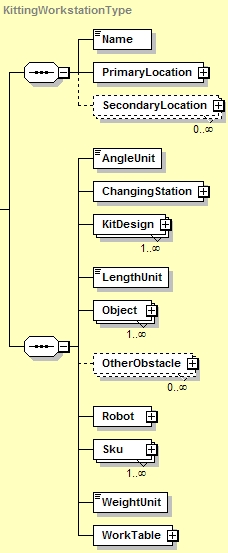
\includegraphics[width=3.166in]{images/kittingModelSmallCropped.jpg}
\caption{Kitting Workstation Model}
\label{fig:WorkstationModel}
\end{figure}

The types (i.e. classes or datatypes) of the attributes of a kitting
workstation are not shown on Figure~\ref{fig:WorkstationModel}. The
structures of several of the attributes are shown on the following figures:
\begin{itemize}
\item ChangingStation -- EndEffectorChangingStationType:
  Figure~\ref{fig:ChangingStation}
\item KitDesign -- KitDesignType: Figure~\ref{fig:KitDesign}
\item Object -- LargeBoxWithEmptyKitTraysType Figure~\ref{fig:LBWEKT},
  LargeBoxWithKitsType Figure~\ref{fig:LBWK}, and PartsTrayWithParts
  Figure~\ref{fig:PTWP}
\item Robot -- RobotType Figure~\ref{fig:Robot}
\item Sku -- StockKeepingUnitType Figure~\ref{fig:SKU}
\item WorkTable -- WorkTableType Figure~\ref{fig:WorkTable}.
\end{itemize}

The type of the Object elements of a kitting workstation is
SolidObject. That is an abstract class not intended to be
instantiated. Hence, the figures \ref{fig:ChangingStation} through
\ref{fig:WorkTable} show the structures of derived classes of
SolidObject that are intended to be used for instances of the Object
attribute.

\begin{figure}[htb!]
\centering
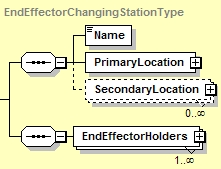
\includegraphics[width=3.166in]{images/changingStation.jpg}
\caption{Changing Station Model}
\label{fig:ChangingStation}
\end{figure}

\begin{figure}[htb!]
\centering
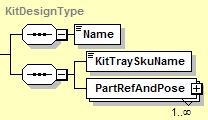
\includegraphics[width=3.1in]{images/kitDesign.jpg}
\caption{Kit Design Model}
\label{fig:KitDesign}
\end{figure}

\begin{figure}[htb!]
\centering
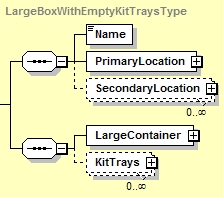
\includegraphics[width=3.1in]{images/largeBoxWithEmptyKitTrays.jpg}
\caption{Large Box With Empty Kit Trays Model}
\label{fig:LBWEKT}
\end{figure}

\begin{figure}[htb!]
\centering
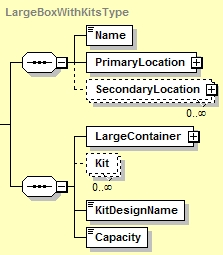
\includegraphics[width=3.1in]{images/largeBoxWithKits.jpg}
\caption{Large Box With Kits Model}
\label{fig:LBWK}
\end{figure}

\begin{figure}[htb!]
\centering
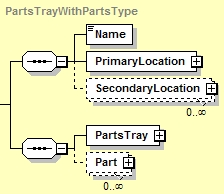
\includegraphics[width=3.1in]{images/partsTrayWithParts.jpg}
\caption{Parts Tray With Parts Model}
\label{fig:PTWP}
\end{figure}

\begin{figure}[htb!]
\centering
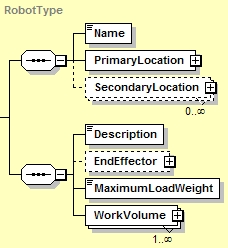
\includegraphics[width=3.166in]{images/robot.jpg}
\caption{Robot Model}
\label{fig:Robot}
\end{figure}

\begin{figure}[htb!]
\centering
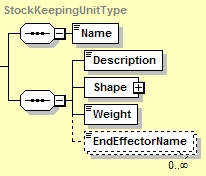
\includegraphics[width=3.166in]{images/sku.jpg}
\caption{Stock Keeping Unit Model}
\label{fig:SKU}
\end{figure}

\begin{figure}[htb!]
\centering
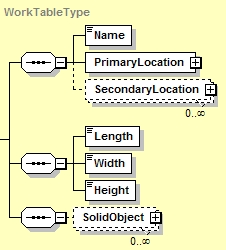
\includegraphics[width=3.166in]{images/worktable.jpg}
\caption{Work Table Model}
\label{fig:WorkTable}
\end{figure}

The robot model is simple and does not currently have any kinematics or
even any shape for the robot. It is likely that additional attributes will
be added in the future.

The kitting workstation model has been fully defined in each of two
languages: XML schema language \cite{Walmsley.2002},
\cite{XMLschemaPrimer}, \cite{XMLschemaStructures}, and Web Ontology
Language (OWL \it sic\rm) \cite{OWLoverview}, \cite{OWLprimer},
\cite{OWLspec}. Further information on the implementations may be
found in Section \ref{Implementation}. 

\subsection{Robot Requirements}
As mentioned earlier, the plan format being used is a sequential list of
actions for a robot to perform. The authors devised a ``canonical robot
command'' language in which such lists can be written. The purpose of the
canonical robot command language (CRCL) is to provide generic commands that
implement the functionality of typical industrial robots without being
specific either to the language of the planning system that makes a plan or
to the language used by a robot controller that executes a plan.

It was anticipated that planning systems would plan in some language used
by automated planners and that plans made by such systems would be
translated into the canonical robot command language. It was anticipated
also that plans would be executed by a variety of robot controllers using
robot-specific languages for input programs. The authors themselves are
using a PDDL planner \cite{PDDL} to generate plans in PDDL output language
and are using a ROS controller \cite{ROS} to control a robot. Those two
systems are connected using files of robot commands in CRCL. After a plan
has been generated by the PDDL planner, the plan is translated into a CRCL
file. When the plan is being executed, the CRCL commands are translated
into ROS commands.

In order to support this mode of operation, the basic robot and robotic
workcell must meet certain requirements. These include:

\begin{itemize}
\item A robot suitable for use with CRCL commands has one arm and can position
and orient the end of the arm anywhere in some work volume within some
tolerance. At each point in the work volume, the range of orientations that
can be attained may be limited.

\item The speed and acceleration of the end of the arm may be controlled.

\item A robot can attach one end effector at a time to the end of the arm from an
end effector changing station and can detach the end effector at the
changing station. The changing station itself is passive.  Attaching an end
effector is done by (1) moving the robot arm (with no end effector
attached) to an attachment position with respect to an end effector and (2)
giving a CloseToolChanger command. Detaching an end effector is done by (1)
moving the robot arm (with an end effector attached) to a detachment
position and (2) giving an OpenToolChanger command. The attachment and
detachment positions are normally at an end effector changer in the end
effector changing station.

\item All end effectors available to the robot are stored in the end effector
changing station.

\item All end effectors are assumed to be grippers.

\item All grippers have two states, open and closed. A gripper can hold an
object in the closed state and cannot hold an object in the open
state. [Additional states may be added later, such as open a certain
distance or closed with a certain force.]

\item Opening or closing any gripper mounted at the end of a robot arm is
exercised by giving a command to the robot.

\item The robot cannot simultaneously move and open or close the gripper.

item There is always a controlled point. When no end effector is on the arm,
the controlled point is at the end of the arm. When an end effector
is mounted on the end of the arm, the controlled point is the tool
center point.

\item The robot can move the controlled point smoothly through a series of
poses from a start pose at which it is not moving to an end pose at
which it is not moving, provided that all poses are given before
motion starts. The acceleration and steady state speed of the
controlled point may be specified. The robot will do its best to
maintain the requested steady state speed but may reduce (but not
increase) speed or acceleration as necessary to allow for the dynamics
of arm motion.

\item A tolerance for the intermediate points of a smooth motion may be set.
The controlled point must pass the intermediate points within the
given tolerance (without coming back to a point after missing it by
more than the tolerance).
\end{itemize}

The CRCL includes commands for a robot controller. In normal system operation,
CRCL commands will be translated into the robot controller's native
language by the robot's plan interpreter as it works its way through a
CRCL plan. One CRCL command may be interpreted into several native
language commands.
One or more canonical robot commands may be placed on a queue and
executed (in order) when desired. Several additional assumptions are
made on the execution behavior of the robot controller. These include:

\begin{itemize}
\item If the robot controller is unable to execute a particular instance of a
canonical robot command, subsequent behavior is up to the robot
controller.

\item The pose at the end of a command is called the current pose.

\item While a plan is being executed, the robot should not move except as
directed by a canonical robot command.

\item Status of command execution is not returned by the robot controller to
the plan interpreter (or any other command generator).

\item The default coordinate system for poses used in the canonical robot commands is
the workstation coordinate system. This may be changed through the use of
a CRCL command to be either the workstation coordinate system, the
robot base coordinate system, or the tool-tip coordinate system.
\end{itemize}

The exact syntax of the CRCL commands is provided in Section \ref{sect:Implementation.CRCL}.
